\documentclass[iop, usenatbib]{emulateapj}

\usepackage[T1]{fontenc}
\usepackage[utf8]{inputenc}
\usepackage[english]{babel}

%\usepackage[varg]{txfonts}
\usepackage{amssymb}
\usepackage{amsmath}
\usepackage{epsfig}
\usepackage{graphics}
\usepackage{amsmath}
\usepackage{color}
%\usepackage{xifthen}

%Debug addition for collaborators
%\usepackage[switch, displaymath, modulo]{lineno}
%\linenumbers
%%\renewcommand\linenumberfont{\color{red}\normalfont\tiny\sffamily}
%\renewcommand\linenumberfont{\normalfont\tiny\sffamily}
%\usepackage{natbib,twoopt}


%Collides with emulateapj
%%%%%%%%%
%\usepackage{siunitx}
% Units
%\DeclareSIUnit{\erg}{erg}
%%%%%%%%%


%Commands
\newcommand{\be}{\begin{equation}}
\newcommand{\ee}{\end{equation}}
%\newcommand{\bea}{\begin{eqnarray}}
%\newcommand{\eea}{\end{eqnarray}}
%\newcommand{\bea}{\begin{align}\begin{split}}
%\newcommand{\eea}{\end{split}\end{align}}
\newcommand{\ud}{\text{d}}

%normal 3-vectors
%\renewcommand{\vec}[1]{\ensuremath{\mathbf{#1}}}
\renewcommand{\vec}[1]{\ensuremath{\boldsymbol{#1}}}

%four-vectors
\makeatletter
\def\fvec#1{\underline{\sbox\tw@{$#1$}\dp\tw@\z@\box\tw@}}
\makeatother

%higlight color
\newcommand{\red}[1]{\textcolor{red}{#1}}

%general shortcuts
\newcommand{\pd}{\ensuremath{\partial}} %partial derivative
\newcommand{\rg}{\ensuremath{r_{\mathrm{g}}}}
\newcommand{\Req}{\ensuremath{R_{\mathrm{e}}}}
\newcommand{\sch}{Schwarzschild }
\newcommand{\Ca}{\ensuremath{\mathcal{C}}}

\newcommand{\rb}{\ensuremath{\bar{r}}}
\renewcommand{\ub}{\ensuremath{\bar{u}}}
\newcommand{\wb}{\ensuremath{\bar{\omega}}}
\newcommand{\Ob}{\ensuremath{\hat{\Omega}}}
\newcommand{\nub}{\ensuremath{\bar{\nu}}}
\newcommand{\zetab}{\ensuremath{\bar{\zeta}}}
\newcommand{\Bb}{\ensuremath{\bar{B}}}
\newcommand{\mub}{\ensuremath{\bar{\mu}}}

\newcommand{\vw}{\ensuremath{v_{\omega}}}
\newcommand{\vz}{\ensuremath{v_{\mathrm{Z}}}}

\newcommand{\Msun}{\ensuremath{M_{\odot}}}

\newcommand{\lgamma}{\gamma_{\text{L}}}

%%%%%%%%%%%%%%%%%%%%%%


\slugcomment{ }
\shorttitle{Radiation from rotating oblate neutron stars}
\shortauthors{Nättilä \& Pihajoki}

\voffset=-1cm

\begin{document}
\title{Radiation from rotating oblate neutron stars}

\author{J. Nättilä\altaffilmark{1,2}\thanks{nattila.joonas@gmail.com},
  P. Pihajoki\altaffilmark{3}}
%  J. Poutanen\altaffilmark{1,2}}

\affil{}
\altaffiltext{1}{Tuorla Observatory, University of Turku}
\altaffiltext{2}{NORDITA, Stockholm}
\altaffiltext{3}{University of Helsinki}


\begin{abstract}
We derive a framework of formulae useful for computing emission from and
around compact rotating objects, focusing on emission from rotating
neutron stars. We use a surrounding spacetime metric that takes rotation
into account to second order.  Similarly, we take the oblate shape of
the star into account to second order as well. The entire framework is
derived in a fully general relativistic manner, and as such we also
validate previous ad-hoc special relativistic formulations during the
derivation.  As an application and to validate our results, we use the
machinery to calculate accurate pulse profiles from hot spots around
rapidly rotating neutron stars.
\end{abstract}
\keywords{stars: neutron}

\section{Introduction}
Accurate modelling of the emission from and around compact objects is a
complicated combination of radiative processes and relativity.  Not only
is the object bending the spacetime around it, and hence affecting the
trajectory of photons, but also affecting the apparent observed
radiation via fast rotation and relativistic surface velocities.
Applications for such accurate analysis of the radiation range from
numerous black hole disk emission studies to neutron star (NS) pulse
profile analysis.  Emission around rotating (Kerr) black holes has been
conveniently implemented and formulated in the publicly available \textsc{geokerr} and
\textsc{grtrans} codes \citep{dexter2009,dexter2016}.
On the other hand, a further complication with neutron stars is that the
emission is not only originating from the viscinity of the object but
from the surface of the star itself.  Hence, computing accurate pulse
profiles from e.g. hot spots rotating around rapidly spinning neutron
stars has been under a lot of scrutinity recently, because of many
upcoming or planned new spaceborne observatories like ESA's
\textit{XIPE} or NASA's \textit{NICER} X-ray missions.
When accurate observations become readily available,
modelling the pulse profiles will become a new and formidable tool in
exploring neutron star physics, for example as a way to constrain the as yet unknown neutron star  
equation of state (EoS).

intro 
    - applications
literature
    - forward-in-time
    - backwads-
the gap
why?
    physics check
    GR gives correct results
    - slower but faster than full 2nd order geodesic eq
    visualization
paper outline


\clearpage



%________________________________________________________________
\section{Theory}

\subsection{Space-time metric}

\begin{table*}[ht!]
  \label{tab:coeffs}
%\renewcommand{\arraystretch}{1.4}
\begin{center}
\caption{Series expansion terms of the metric coefficients up to $\Ob^2$}
%\begin{small}
\begin{tabular}{l c c c c}
  \hline
  \noalign{\vskip 0.5ex}
              &  $\Ob = 0$  &  $\Ob^1$   & $\Ob^2$  &  error  \\
  \hline
  \noalign{\vskip 2ex}
  $\nub$       &  $\displaystyle \log\left[ 1-\frac{\ub}{2}\right] - \log\left[ 1+\frac{\ub}{2} \right]$ & --- & $\displaystyle +\left(\frac{\beta}{3}-qP_2(\cos\theta) \right)\ub^3 $ & $+\mathcal{O}\left(\Ob^2 \times \ub^4 \right)$ \\[3ex]
  $\Bb$         &  $\displaystyle \left( 1-\frac{\ub}{2} \right) \left(1+\frac{\ub}{2} \right)$ & --- & $\displaystyle+\beta \ub^2$ & $+\mathcal{O}(\Ob^4) \times \mathcal{O}(\ub^4)$ \\[3ex]
  $\zetab$     &  $\displaystyle \log\left[ \left( 1-\frac{\ub}{2} \right) \left(1+\frac{\ub}{2} \right) \right]$ & --- & $\displaystyle +\beta \left( \frac{3}{4}P_2(\cos{\theta}) - \frac{1}{3} \right) \ub^2$ & $+\mathcal{O}(\Ob^2) \times \mathcal{O}(\ub^4)$ \\[3ex]
%  $\wb$       & --- &  $\displaystyle \frac{2G\mathcal{J}}{c^2\rb^3}$ & $\displaystyle -\frac{3}{2}\ub + \mathcal{O}(\ub^2)$ & $+\mathcal{O}(\Ob^3)$ \\[2ex]
  $\wb$       & --- &  $\displaystyle \wb_1 \ub^3 $ & $\displaystyle -3\wb_1 \ub^4 $ & $+ \mathcal{O}(\Ob^3) + \wb_1 \ub^3 \times \mathcal{O}(\ub^2)$ \\[2ex]
  \hline
\end{tabular}
\begin{center}{ 
    Note:
    The angular velocity term of the local inertial frame is simplified by the notation $\wb_1 \equiv 2c^4 j/G^2 M$.
}
\end{center}
%\end{small}
\end{center}
\end{table*}


The spacetime metric around a static non-rotating spherically symmetric object is given by the well known \sch solution
\begin{align}\begin{split}
ds^2 & = -(1-u)dt^2 + \\
     & (1-u)^{-1}dr^2+r^2(d\theta^2+\sin^2\theta d\phi^2)
\end{split}\end{align}
where $u = 2GM/c^2 r$ is the dimensionless compactness factor and $r$ is
the radial coordinate, defined so that an area of a sphere in this coordinate system is the usual $4\pi r^2$ at some fixed time.
This is equivalent to an alternative solution known as isotropic \sch metric \citep[see e.g.][]{MTW73}
\begin{align}\begin{split}
\label{eq:ISch}
ds^2 & = -\left( \frac{1-\frac{\ub}{2}}{1+\frac{\ub}{2}} \right)^2 dt^2 + \\
     & (1+\frac{\ub}{2})^4(d\rb^2 + \rb^2(d\theta^2+\sin^2\theta d\phi^2)),
\end{split}\end{align}
where  $\rb$ and $\ub=GM/c^2\rb$ are the so-called isotropic radial
coordinate and the corresponding isotropic compactness factor,
respectively. 
%defined so that the circumference of a circle in this metric is $2\pi\rb$.
This kind of isotropic metric has the useful feature that surfaces of constant time are conformally flat, and hence the angles are represented without distortion.
%In this kind of isotropic metric the angles in the constant time hyperslices are represented without distortion, hence the name of the metric.
This, however, also means that isotropic coordinates do not faithfully represent the distances within the spheres nor does the radial coordinate correspond directly to the radial distance.
From here on, we mark all variables related to the isotropic radial coordinate with a bar on top.
%The relation between these two radial coordinates can be easily seen to be $r = \rb(1+\ub)^2$.

Let us consider a rotating compact object.
In addition to the dimensionless compactness factor $u(r)$ (or
$\ub(\rb)$), to describe our system
we need a dimensionless angular velocity
\be
\Ob = \Omega \left( \frac{\Req^3}{G M} \right)^{1/2},
\ee
where $\Omega$ is the angular velocity of a sphere with an equatorial
radius $\Req$ and a mass $M$ scaled with a Newtonian mass shedding
(Kepler) limit $(GM/\Req^3)^{1/2}$ \citep[see][p.29]{rcs}.  Here $\Req$
is described using the usual \sch radial coordinate and corresponds to
the equatorial radius of the star for which $2\pi\Req$ gives the proper
length of the circumference.  The asymptotically flat metric near a
stationary axisymmetric rotating object in isotropic form is
\citep{BW71} 
%\bea
\begin{align}\begin{split} \label{eq:BWmetric}
ds^2 & = -e^{2\nub}c^2dt^2 +
     \rb^2 \sin^2\theta \Bb^2 e^{-2\nub}(d\phi - \wb cdt)^2 + \\
     & e^{2(\zetab-\nub)}(d\rb^2 + \rb^2d\theta^2),
\end{split}\end{align}
%\eea
where $\wb$ is the angular velocity of the local inertial frame and the functions $\nub$, $\Bb$ and $\zetab$ in the metric coefficients can be expanded in the powers of $\Ob$ and $\ub$ \citep{BI76}.
%\red{rcs:14}
%\red{rcs:15}
Here $e^{-\nub}$ is the time dilation factor relating the proper time of the local observer to the time at infinity.
Physical interpretation of $\Bb$ follows from the fact that the proper circumference of a circle around the axis of symmetry is $2\pi(e^{-\nub} \Bb \rb \sin\theta)$.
Similarly, the interpretation of $\zetab$ follows from the fact that $e^{\zetab - \nub}$ acts as a conformal (angle preserving) factor of the spacetime. %determining the orthogonality of the 2-surfaces.
The zeroth terms of the series expansions ($\Ob = 0$) are the familiar isotropic \sch metric coefficients (see Table \ref{tab:coeffs}).
%\be
%e^{\nu_0} = (1-\ub/2)/(1+\ub/2),
%\ee
%\be 
%\Bb_0 = (1-\ub/2)(1+\ub/2)
%\ee
%and
%\be
%\zetab_0 = \log \Bb_0.
%\ee

The first order expansion in rotation ($\Ob^1$) is formally related to Kerr metric.
In this case we introduce an angular velocity term of the local inertial frame $\wb$ that accounts for the frame-dragging effects. %\red{rcs:13}
Up to first order, this can be defined as
\be
\wb = \frac{2c^4j}{G^2M}\ub^3,
\ee
where the dimensionless quantity $j=\mathcal{J}/M^2$ and $\mathcal{J} = I \Omega$ is the star's angular momentum with moment of inertia $I(M,\Omega)$.

Finally, the second order expansion ($\Ob^2$) correspond to a similar
approximation as the Hartle-Throne slow-rotation spacetime, which
introduces quadrupole moments into the metric.  These second order
multipole moments can be defined via dimensionless quantities $q$ and
$\beta$ that are the dimensionless moments of energy density and
pressure.  \citet{aGM14} defined an approximate relation for these
parameters based on their computations of rotating NSs with various
different EoSs.  Due to the NS spacetime being almost hairless we can
parameterize these quantities with great accuracy by using only the
dimensionless angular velocity $\Ob$ and compactness factor
\be
x = \frac{G M}{c^2 \Req}.
\ee
Note that both of these parameters are defined via the equatorial
circumferential radius $\Req$ defined in the usual \sch radial coordinate
system.
To the lowest order, these approximations are
\be
q = -0.11 \frac{\Ob^2}{x^2},
\ee
\be
\beta = 0.4454 \Ob^2 x,
\ee
and
\be
I = \sqrt{x} (1.136 - 2.53 x + 5.6 x^2) M \Req^2.
\ee
Note also that both $q$ and $\beta$ are $\mathcal{O}(\Ob^2)$, while $I$ is $\mathcal{O}(\Ob)$.
    
It is possible to transform between the usual $r$ and the isotropic $\rb$
coordinates using the relation \citep{FIP86}
\be\label{eq:rb2r}
r = \Bb e^{-\nub} \rb.
\ee
The relation between the two infinitesimal radial coordinates turns out to be
\be\label{eq:drb2dr}
dr = e^{\zetab} d\rb,
\ee
which can be computed using the series presentation of \cite{BI76}.

Since the series expansions of the metric coefficients are expanded
using the isotropic radial coordinate $\rb$, we will favor this notation
in our derivation.  However, in some cases we will simplify the
equations into more intuitive form by using the areal $r$ coordinate.
%As such, some caution is needed when dealing with the radial coordinates.

%The metrics of the rotating isoradial spacetime is then
%\begin{align}\begin{split}\label{eq:isorad}
%ds^2 & = -e^{2\nub}c^2dt^2 +
%     r^2 \sin^2\theta (d\phi - \bar{\omega}cdt)^2 + \\
%     & e^{-2\nub}dr^2 + e^{2\mu}r^2d\theta^2),
%\end{split}\end{align}
%where $e^{2\mu} = e^{2\zetab}/\Bb^2$.
%TODO: physical explanation of the metric functions

\subsection{Oblate shape of the neutron star}

\begin{figure}
\centering
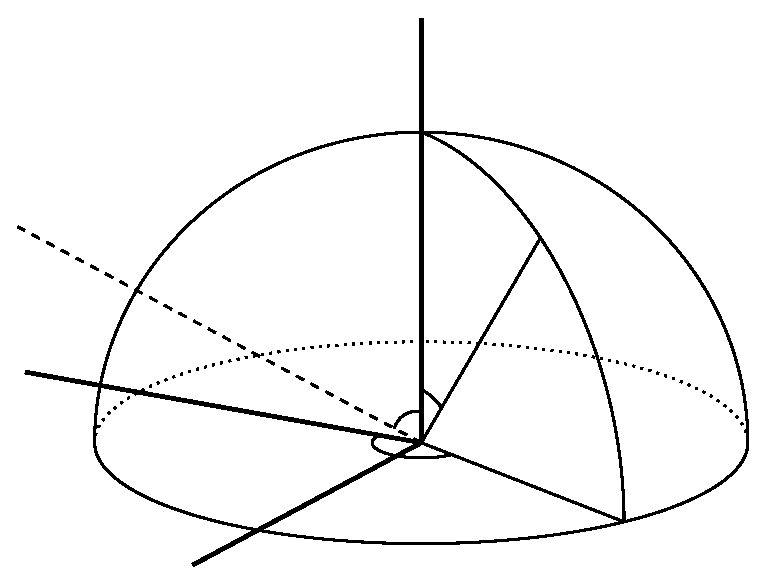
\includegraphics[width=7cm]{figs/fig1.eps}
\caption{\label{fig:geom}
  Geometry of the system.
}
\end{figure}


Due to rotation and finite pressure supporting it, the neutron star is
not a perfect sphere when it is rotating.  It, however, retains
axisymmetry, and can be approximated with an oblate spheroid.  Similarly
to the second order space-time quantities,
\citet{aGM14} derived an approximate shape of a rotating neutron star by
expressing the radius as a function of colatitude $\theta$, yielding
\begin{align}\begin{split}\label{eq:radf}
    R(\theta) &= \Req \left( 1 - \frac{\Req - R_{\mathrm{p}}}{\Req} \cos^2\theta \right) \\
              &= \Req (1-\Ob^2 (0.788 - 1.03x) \cos^2 \theta,
\end{split}\end{align}
where $R_{\mathrm{p}}$ is the radius on the rotational axis and $R(\pi/2) = \Req$ is the equatorial circumferential radius measured in the usual \sch metric. 
Elemental surface area for a spheroid is given as (using the areal radial coordinates)
\be
dS(\theta) = R^2(\theta) \sin\theta \sqrt{1 + f(\theta)^2}d\theta d\phi,
\ee
where
\be
f(\theta) = \frac{1}{\bar{R}(\theta)} \frac{d \bar{R}(\theta)}{d \theta} 
= \Bb e^{-\zetab-\nub} \frac{1}{R(\theta)} \frac{dR(\theta)}{d\theta}, 
\ee
and $\Bb e^{-\zetab-\nub} \approx \left(1-\frac{2 G M}{c^2 r}\right)^{-1/2} + \mathcal{O}(\Ob^2)$.
The angle $\gamma$, defined as the angle between the radial unit vector
$\vec{r}$ and the surface normal $\vec{n}$, is given by
\be
\cos\gamma = \left(1 - f(\theta)^2\right)^{-1/2}.
\ee
Then the normal to the surface can be defined using the radial vector $\vec{r}$ and the tangential vector $\vec{\theta}$ as
\be
\vec{n} = \cos\gamma \vec{r} + \sin\gamma \vec{\theta}.
\ee
See also Fig.~\ref{fig:geom} for a clarification of the angles.
From here it is again clear how the angles transform easily in the isotropic metric while the quantities related to the area are simplified in the usual \sch metric.

\subsection{Geodesic motion through Hamilton-Jacobi equation}
Geodesic motion in space-time characterized by a metric
$g_{ij}$ is governed by Hamilton-Jacobi equation
\be\label{eq:hamjac}
2\frac{\pd S}{\pd \tau} = g^{ij} \frac{\pd S}{\pd x^i}\frac{\pd S}{\pd x^j},
\ee
where $g^{ij}$ is the inverse metric and $S$ denotes the Hamilton's principal function.
For the two Killing vectors $k_{t}^{\alpha} = (1,0,0,0)$ (asymptotic
time symmetry) and $k_{\phi}^{\alpha} = (0,0,0,1)$ (rotation symmetry
along azimuthal angles) in the rotating space-time, the Frobenius
theorem implies the existence of a family of 2-surfaces orthogonal to
these vectors \citep[see e.g][p.12]{rcs}.  This means that there are
surfaces of constant $t$ and $\phi$ in our spacetime, yielding two constants of
motion, energy $E$ and the $z$-component of the angular momentum, $L_z$.  
We then seek a solution of equation~\eqref{eq:hamjac} in the form
\be
S = \frac{1}{2}\delta_1 \tau - Et + L_z\phi + S_{\rb}(\rb) + S_{\theta}(\theta).
\ee
With the metric function \eqref{eq:BWmetric} this becomes
%\begin{align}\begin{split}
%2 r^2 \delta_{1} =~ & e^{2\nub} r^2 \pd_r^2 - e^{-2\nub} r^2 (E-L_z \omega)^2 \\
%& + e^{-2\mu} \pd_\theta^2 + \frac{L_z^2}{\sin^2 \theta},
%\end{split}\end{align}
\begin{align}\begin{split} 
    \delta_1 \rb^2 \Bb^2 e^{-2\nub} =~& \rb^2 \Bb^2 e^{-2\zetab} \pd_{\rb}S_{\rb}S^2 - e^{-4\nub} \Bb^2 \rb^2 (E - L_z \wb)^2 \\
                                & + \Bb^2 e^{-2\zetab} \pd_{\theta}S_{\theta}^2 + \frac{L_z^2}{\sin^2\theta}.
\end{split}\end{align}
After re-organizing terms and introducing a simplifying notation
$e^{\zetab}/\Bb \equiv e^{\mub}$ we get
\begin{align}\begin{split}\label{eq:S}
& e^{-2\mub}\pd_{\theta}S_{\theta}^2 + \frac{L_z^2}{\sin^2\theta} = \\ 
& \Bb^2 e^{-2\nub}\rb^2 \left[ e^{2(\nub-\zetab)} \pd_{\rb}S_{\rb}^2
-\delta_{1} - e^{-2\nub}(E - L_z \wb)^2\right],\\
\text{TARKASTA SULKEET -Pauli}
\end{split}\end{align}
%By using the isoradial coordinate $r$ and notation $e^{\zetab}/\Bb \equiv e^{\mu}$ this can be simplified to
%\begin{align}\begin{split}
%    \delta_1 r^2 &- e^{2\nub} r^2 \pd_rS^2 \\
%                &+ e^{-2\nub} r^2 (E+L_z \wb)^2 = e^{-\mu} \pd_{\theta}S^2 + \frac{L_z^2}{\sin^2\theta},
%\end{split}\end{align}
that already hints towards separability only if $\nub = \nub(\rb)$, $\Bb = \Bb(\rb)$, $\zetab = \zetab(\rb)$ and $\mu = \mu(\theta)$.
To first order in rotation, i.e. $\mathcal{O}(\Ob)$, this condition is
satisfied exactly because $e^{\mub} = 1 + \mathcal{O}(\Ob^2)$, in
addition to $\Bb = \Bb_0(\rb) + \mathcal{O}(\Ob^2)$ and $\Bb =
\Bb_0(\rb) + \mathcal{O}(\Ob^2)$ (see Table \ref{tab:coeffs}).  In the
second order of the expansion, $\theta$ dependent mass and pressure
quadrupole moments are present, and separability is lost.
For geodesics, however, these higher order deviations only
contribute very close to the actual NS surface, and 
neglecting them enables us to obtain accurate approximations of the
photon path.
%\red{rcs:66}
%However, the deviations are rather small and for $\mathcal{O}(\Ob^2)$ pressure(?) quadrupole moment is negliblible after which we are left with  mass quadropole moment only.
%In this case the dependence of $r$ and $\theta$ are present through $e^{\nub}$ terms but $e^{\mu} \approx 1$ still.
Since we only consider null geodesics, we could set $\delta_1 = 0$ at
this point, but for reasons of generality, this substitution is not made.

If we now assume separability, we can introduce a separation variable
$\Ca$ known as Carter's constant (third constant of motion) in order to
solve the differential equation \eqref{eq:S}.  By noting that the
conjugate momenta correspond to the first derivatives of $S$ with
respect to the generalized coordinates, we can write the components of 
four-momentum, \fvec{p}, as
\begin{align}
  p_t        &= -E \label{eq:p_t}\\
  p_{\rb}    &= \pm e^{\zetab - 2\nub} \left( \delta_1 e^{2\nub} + (E - L_z \wb)^2 - \frac{\Ca}{\Bb^2 e^{-4\nub} \rb^2} \right)^{1/2}\label{eq:p_r}\\
  p_{\theta} &= \pm e^{\mub} \left( \Ca - \frac{L_z^2}{\sin^2\theta} \right)^{1/2}\label{eq:p_the}\\
  p_{\phi}   &= L_z\label{eq:p_p}.
\end{align}
Similarly, we the components of a local tetrad frame are
\begin{align}
  p^{(t)} &= -p_{(t)} = -e_{(t)}^{\hat{\mu}} p_{\hat{\mu}} = -e^{-\nub}p_t \label{eq:tetp_t}\\
  p^{(\rb)} &= p_{(\rb)} = e_{(\rb)}^{\hat{\mu}} p_{\hat{\mu}} = e^{-\zetab + \nub} p_{\rb} \label{eq:tetp_r}\\
  p^{(\theta)} &= p_{(\theta)} = e_{(\theta)}^{\hat{\mu}} p_{\hat{\mu}} = \frac{1}{\rb} e^{-\zetab+\nub} p_{\theta} \label{eq:tetp_theta}\\
  %p^{(\phi)} &= p_{(\phi)} = e_{(\phi)}^{\hat{\mu}} p_{\hat{\mu}} = -e^{-\nub} \wb p_t + \frac{1}{r \sin\theta} p_{\phi} \label{eq:tetp_phi},
  p^{(\phi)} &= p_{(\phi)} = e_{(\phi)}^{\hat{\mu}} p_{\hat{\mu}} = \frac{1}{e^{-\nub} \Bb \rb \sin\theta} p_{\phi} \label{eq:tetp_phi},
\end{align}
where $e^{\hat{\mu}}_{(a)}$ with index $a = t, \rb, \theta$ and $\phi$ are the tetrads of metric \eqref{eq:BWmetric}.


\subsection{Ray tracing photons}
Radiation is emitted from the surface of a star at an emission point
$(r_e,\theta_e,\phi_e)$.  The radiation travels along a geodesic with a
specific intensity $I_{\nu}$ as measured by an observer co-moving with
the emission point.  The radiation is observed at an image plane
situated at a radial distance $r$, with $r\rightarrow\infty$.  We then
wish to calculate the projected image of the star at this image plane.

First we set up the coordinate system so that the plane of observation
is towards $\phi = 0$ and $\theta = i$, where $i$ is the angle of
inclination.  The geodesic will be emitted with a four-momentum
$\fvec{p}_e$, and if it is eventually observed at the image plane at
infinity, it will have a final four-momentum of $(E,\hat{p}_r,0,0)$,
purely in the radial direction.  Likewise, the components of the
position must satisfy
\begin{align}
\theta &\rightarrow i \\
\phi   &\rightarrow 0,
\end{align}
as $r\rightarrow\infty$.
The change in the time and angular components along the geodesic can be written as
\begin{align}
dt      &= \frac{p^t}{p^{\rb}}\ud \rb \label{eq:deltatime} \\
d\theta &= \frac{p^\theta}{p^{\rb}}\ud \rb \label{eq:deltatheta} \\
d\phi   &= \frac{p^\phi}{p^{\rb}}\ud \rb \label{eq:deltaphi},
%d\theta &= \int_{r_e}^\infty \frac{p^\theta}{p^r}\ud r \label{eq:deltatheta} \\
%d\phi   &= \int_{r_e}^\infty \frac{p^\phi}{p^r}\ud r \label{eq:deltaphi},
\end{align}
with a total change of angles $\Delta\theta$ and $\Delta\phi$ when integrating from $r_e$ to $\infty$.
The condition for being observed is then
\begin{align}
\theta_e + \Delta\theta &= i \label{eq:thetacond}\\
\phi_e + \Delta\phi     &= 0 \label{eq:phicond}.
\end{align}

The projected image of the star on the image plane can then be described by two celestial coordinates:
abscissa $\hat{x}$ and ordinate $\hat{y}$.
Making use of the tetrad components
\eqref{eq:tetp_t}--\eqref{eq:tetp_phi}, we obtain \citep[][p.347]{cha}
\be\label{eq:xhat}
\hat{x} = \left( \frac{rp^{(\phi)}}{p^{(t)}} \right)_{r \rightarrow \infty} = \frac{1}{\sin i} \frac{L_z}{E}
\ee
and
\be\label{eq:yhat}
\hat{y} = \left( \frac{rp^{(\theta)}}{p^{(t)}} \right)_{r \rightarrow \infty} = \frac{\sqrt{\Ca - \frac{L_z^2}{\sin^2 i}}}{E}.
\ee
Here it is useful to transform into a polar coordinate system on the
image plane, as the
form of the equations \eqref{eq:xhat} and \eqref{eq:yhat} strongly
suggest a more intuitive form if this is done. In this system
we use as coordinates the radial distance from the center point, or the impact
parameter $b$, and the polar rotation angle $\chi$.  We take $\chi$ to
increase clockwise from the projected spin axis of the neutron star,
with $\chi=0$ corresponding to the projected direction from the south to
the north pole of the neutron star.  We then express the impact
parameter $b$ and the angle $\chi$ via 
$L_z$ and $\Ca$ as%
\footnote{
    Here, the nature of Carter's constant as a generalized squared
    angular momentum is apparent.
%From here, the nature of Carter's constant as a ``general''
%angular momentum (squared) felt by the photon becomes clear when
%considering the usual definition $\vec{I} = \vec{b} \times \vec{p}$,
%where $\vec{I}$ is the angular momentum, $\vec{b}$ is the axis of the
%rotation, and $\vec{p}$ is the (linear) momentum.
}%
\be
b = \frac{\sqrt{\Ca}}{E}
\ee
and
\be
\sin \chi = \frac{1}{\sin i} \frac{L_z}{\sqrt{\Ca}}.
\ee
The constants of motion, combined with the geodesic null condition
$p^\mu p_\mu = 0$, allow us to solve $p^\theta$ and $p^\phi$ in
terms of $\rb$.
%We can then substitute these back into equations \eqref{eq:thetacond} and \eqref{eq:phicond}, to get the implicit solutions for $b$ and $\chi$ as
%\begin{align}
%\theta_e + \Delta\theta &= \Theta(R_e, \theta_e, \phi_e, b, \chi) = i\\
%\phi_e + \Delta\phi     &= \Phi(R_e, \theta_e, \phi_e, b, \chi) = 0.
%\end{align}
As the final step we can substitute the four-momentum components and
image-plane coordinates into \eqref{eq:deltatime}--\eqref{eq:deltaphi}
and solve the system of three first-order differential equations (in
terms of $t$, $\theta$ and $\phi$) with $\rb$ as a variable.
%% \begin{align}\begin{split}
%% %\int_{\mathrm{R_e}}^{\infty} \frac{p^{\phi}}{p^r} dr =
%%  \Delta \phi &= 
%%  \int_{\mathrm{\bar{R}_e}}^{\infty} \frac{ \frac{L_z}{\sin^2\theta} - e^{-2\nub}r^2\wb(E-L_z \omega)}{r^2 \sqrt{(E-L_z\omega)^2-\frac{\mathcal{C}}{e^{-2\nub}r^2}}} dr \\
%%  &= \int_{\mathrm{\bar{R}_e}}^{\infty} \frac{dr}{r^2} \frac{\frac{\sin\chi \sin i}{\sin^2\theta} - e^{-2\nub}r^2\wb \left(\frac{1}{b} + \wb \sin\chi \sin i \right)}{\sqrt{\left(\frac{1}{b} + \wb \sin\chi \sin i \right)^2 - \frac{1}{e^{-2\nub} r^2}}}
%% \end{split}\end{align}

% dphi = phi(r) dr
%\begin{align}\begin{split}\label{eq:dphi}
% d\phi &= 
% \frac{ \frac{L_z}{\sin^2\theta} - e^{-2\nub}r^2\wb(E-L_z \omega)}{r^2 \sqrt{(E-L_z\omega)^2-\frac{\mathcal{C}}{e^{-2\nub}r^2}}} dr \\
% &=  \frac{\frac{\sin\chi \sin i}{\sin^2\theta} - e^{-2\nub}r^2\wb \left(\frac{1}{b} + \wb \sin\chi \sin i \right)}{\sqrt{\left(\frac{1}{b} + \wb \sin\chi \sin i \right)^2 - \frac{1}{e^{-2\nub} r^2}}} \frac{dr}{r^2}
%\end{split}\end{align}
%and

%% \begin{align}\begin{split}
%% %\int_{\mathrm{R_e}}^{\infty} \frac{p^{\theta}}{p^r} dr =
%%     \Delta \theta &=
%%     \int_{\mathrm{\bar{R}_e}}^{\infty} \frac{e^{-\mu}\sqrt{\mathcal{C} - \frac{L_z^2}{\sin^2\theta}}}{r^2\sqrt{(E-L_z\omega)^2-\frac{\mathcal{C}}{e^{-2\nub}r^2}}} dr \\
%%     &= \int_{\mathrm{\bar{R}_e}}^{\infty} \frac{dr}{r^2} \frac{e^{-\mu} \sqrt{1-\left(\frac{\sin\chi \sin i}{\sin\theta}\right)^2}}{\sqrt{\left(\frac{1}{b} + \wb \sin\chi \sin i \right)^2 - \frac{1}{e^{-2\nub} r^2}}}.
%% \end{split}\end{align}
%\begin{align}\begin{split}\label{eq:dtheta}
%    d\theta &=
%    \frac{e^{-\mu}\sqrt{\mathcal{C} - \frac{L_z^2}{\sin^2\theta}}}{r^2\sqrt{(E-L_z\omega)^2-\frac{\mathcal{C}}{e^{-2\nub}r^2}}} dr \\
%    &= \frac{e^{-\mu} \sqrt{1-\left(\frac{\sin\chi \sin i}{\sin\theta}\right)^2}}{\sqrt{\left(\frac{1}{b} + \wb \sin\chi \sin i \right)^2 - \frac{1}{e^{-2\nub} r^2}}} \frac{dr}{r^2}.
%\end{split}\end{align}
%Both expression reduce back to familiar bending equations in (isoradial) Schwarzschild metric when $\wb=0$, $\sin i = 1$ and $\sin\chi = 0$ for $\Delta\theta$ expression or $\sin\chi = 1$ for $\Delta\phi$.
%However, with oblate stars it suffices to notice that the previous equations are further complicated by the fact that $\bar{R}_e = \bar{R}_e(\theta)$ and $\wb = \wb(\rb, \theta)$.


\subsection{Redshift and emission angle}
It is most convenient to define all radiative processes in the co-rotating
frame of the star.
We denote variables define in a frame that is
momentarily comoving with the stellar surface with a prime.  On the
other hand, our observer is stationary and moving along the timelike
Killing vector.  Hence, we need to transform between stationary and
rotating frames by using the 4-velocity of the star's fluid.  In
addition, we need to take into account that a particle released from
infinity with zero angular momentum will acquire nonzero angular velocity
in direction of the star's rotation due to dragging of inertial frames.
Four-velocity of a stationary observer is then $s^{\alpha} =
s^t(t^{\alpha})$, where the normalization factor $s^t =
e^{-\nub}(1-\vw^2)^{-1/2}$ is obtained from $s_{\alpha}s^{\alpha} = -1$,
and the velocity of the frame is 
\be
\vw = \wb \Bb e^{-2\nub} \rb \sin\theta,
\ee
indicating that the angular velocity as measured by an inertial observer at infinity is $s^{\phi} / s^{t} = d\phi/dt = \wb$.

A circular flow can be defined using the timelike and rotational Killing vectors as $s'^{\alpha} = s'^t (t^{\alpha} + \Omega \phi^{\alpha})$, where the normalization factor is defined as $s'^t = e^{-\nub} (1 - \vz^2)^{-1/2}$ determined by $s'_{\alpha}s'^{\alpha} = -1$.
Here the velocity 
\be
\vz = (\Omega - \wb) \Bb e^{-2\nub} \rb \sin\theta,
\ee
can be identified to be the 3-velocity measured in the frame of a zero angular momentum observer, an observer rotating along the frame with a velocity of $\vw$.

%Observed redshift can then be obtained by comparing the energies of the emerging ($E' = u_{\alpha} s^{\alpha}$) and the observed photon ($E = u_{\alpha} o^{\alpha}$).
%Gravitational redshift from the non-rotating frame is given by $1+z_G = -o_{\alpha} u^{\alpha} = e^{\-nub}$ 
The total redshift as measured by an observed at infinity is then given by an inner-product between a photon $u^{\alpha}$ and a 4-velocity of the star's fluid $s'^{\alpha}$.
With these definitions the redshift is
\be
1 + z = -s'_{\alpha} u^{\alpha} = e^{-\nub} ~\delta^{-1},
\ee
consisting of the gravitational part $e^{\nub}$ and of the second Doppler-like term
\be
\delta = \frac{\sqrt{1-\vz^2}}{1 - \Omega L_z}.
\ee


To compute the emission angle we again have to take the rotating frame
into account.  This can be done by introducing a projection operator
$\bar{h}_{ab} = g_{ab} + s'_a s'_b$, which projects 4-vectors from the
non-rotating frame to the rotating frame where the radiative processes
are defined.  As a definition, we can take the emission angle to be the
angle between photon and a spacelike surface normal vector $n_{\alpha} =
(0, \cos\gamma/N_n, \rb \sin\gamma/N_n, 0)$, with normalization $N_n =
e^{\zetab - \nub}$ fullfilling $n_{\alpha}n^{\alpha} = -1$.  When
projected to the rotating-frame we can then obtain the angle from the
generalized dot-product definition between two vectors as
\be\label{eq:gen_angle}
\cos\alpha' = \frac{\bar{h}_{ab}n^a u^b}{(\bar{h}_{ab} n^a n^a)^{1/2} (\bar{h}_{ab} u^a u^b)^{1/2}}.
\ee
Using the metric defined by \eqref{eq:BWmetric} and a photon with components as \eqref{eq:p_t}$-$\eqref{eq:p_p}, we obtain
\be
\cos\alpha' = \delta e^{2\nub-\zetab} \left[ p_{\rb} \cos\gamma + \frac{p_{\theta} \sin\gamma}{\rb} \right].
\ee
Here it suffices to notice that we are only interested in the emission angle value at the surface of the star i.e. $\rb = \bar{R}(\theta)$.
The result here is similar to the emission angle obtained with a
special-relativistic approahc, using flat-space trigonometry and
Lorentz-boosting to the rotating frame \citep[see e.g.][]{PB06}.

\subsection{Emission}
Observed flux at photon energy $E$ from a small area on an image plane is
\be
dF_E = I_E d\Omega_o,
\ee
where $I_E$ is the specific intensity of the radiation at infinity and
$d\Omega_o$ is the solid angle subtended by the element as measured by
the observer. The total flux is then
the integral of these elements over the image plane. As a
final step this observed flux hast to be connected to the actual
emerging radiation.

The relation between the emergent energy $E'$ to the observed energy $E$ is $E/E' = (1 + z)^{-1}$.
The connection between the monochromatic observed and local intensity is then (see e.g. \citealt{MTW73}, p.588; \citealt{RL79}, p.145)
\be
I_E = \left( \frac{E}{E'} \right)^3 ~I'_{E'}(\alpha'),
\ee
where $I'_{E'}(\alpha')$ is the intensity computed in the frame comoving with the emitting area.
The radiation here is emitted to the direction of the emission angle $\alpha'$ defined in the local rotating frame.
Integrating over the energies, we get the bolometric intensity
\be
I = \left(\frac{E}{E'} \right)^4 ~I'(\alpha').
\ee
The total (monochromatic) flux as a function of observer's time $F_E(t)$ can then be obtained by integrating over the whole image
%\begin{align}\begin{split}
\be\label{eq:fluxint}
F_E(t) = \int I_{E}(t) ~d\Omega_o = \int\int \frac{I'_{E'}(t_*, \alpha')}{(1+z)^3}  ~bdb \, d\chi,
\ee
%\end{split}\end{align}
where $t_* = t - \Delta t$ is the time when the photon was originally
emitted. This can be computed when we know the total travel time $\Delta
t$ against some reference photon, for example the one with the shortest
path to the observer.
\red{discussion about rotating the star and invariance of dt*dphi}

All of these quantities on the star's spherical coordinate system $(\theta, \phi)$ are then mapped to the observers polar image coordinates $(b, \chi)$ via raytracing.
This mapping $(b, \chi) \rightarrow (\theta, \phi)$ allows us to then evaluate the physical quantities
\begin{align}
    \red{\text{Ovatko nämä tarpeellisia? -Pauli}} \\
1+z                  &\rightarrow 1+z(\theta, \phi) \rightarrow 1+z(b, \chi), \\
\cos\alpha'          &\rightarrow \cos\alpha'(\theta, \phi) \rightarrow \cos\alpha'(b, \chi), \\
\Delta t             &\rightarrow \Delta t(\theta, \phi) \rightarrow \Delta t(b, \chi), \\
I'_{E'}(t_*, \alpha') &\rightarrow I'_{E'}(t_*, \cos\alpha'; \theta, \phi) \rightarrow I'_{E'}(t_*, \cos\alpha'; b, \chi)
\end{align}
in the observers plane for the flux calculations.

\subsection{Coordinates in the co-rotating frame}
As was discussed earlier, all of the radiative processes are defined in
the co-rotating frame of the star's surface as it is always the source
of the emission. \red{Mutta abstrakti/intro väittää, että halutaan
    laskea emissiota myös kompaktien kohteiden läheltä, ei vain
pinnalta?} 
Because of this, it is natural to define the shape of
the emitting region using the coordinate system of the co-rotating
observer.  In practice, this then gives us the
integration limits of equation \eqref{eq:fluxint}.

Transformation from the non-rotating frame to the rotating frame can be obtained using a projection operator $\bar{h}_{ab}$ defined previously.
%\be
%\bar{h}_{ab} = g_{ab} + s_a s_b
%\ee
%where $s_a$ is the 4-velocity of the previously defined star's fluid element.
Our metric tensor for the rotating observer is then
\be
\bar{h}_{ab} dx^a dx^b = e^{2(\zetab - \nub)} (d\rb^2 + \rb^2 d\theta) + \frac{\Bb^2 e^{-2\nub} \rb^2 \sin^2\theta}{1-v_Z^2} d\phi_*^2,
\ee
where we have defined a new angular coordinate $\phi_* = \phi - \Omega t$ that is used by the rotating observer.%
\footnote{We thank S. Morsink for pointing this out. 
The normalized longitudinal coordinate ensures that both, rotating and stationary observer, agree that a circle drawn around the star has $2\pi$ radians.}
This new longitudinal coordinate is also seen to be Lorentz contracted by $\gamma_\mathrm{L} = (1-\vz^2)^{-1/2}$ factor.

Next we move to a normal (areal) \sch coordinate system so that emission
regions with similar coordinate extents at different latitudes have the
same area.
By using the equations \eqref{eq:rb2r} and
\eqref{eq:drb2dr} we obtain a longitudinally Lorentz-boosted metric
tensor 
\be \label{eq:gammaSch} 
h_{ab} dx^a dx^b = e^{-2\nub}dr^2 + \frac{e^{2\zetab}}{\Bb^2} r^2 d\theta + \lgamma^2 r^2 \sin^2\theta d\phi_*^2, 
\ee 
where $\gamma_\text{L}$ is the Lorentz boost factor.
The result agrees with (areal) \sch coordinate
system up to first order in rotation due to the fact that $e^{\zetab}/\Bb \approx 1 +
\mathcal{O}(\Omega^2)$.  Additionally we can drop the gravitational
redshift term $e^{-2\nub}$ of the radial coordinate as we are only
considering unit vectors later on.

In order to define a disc-like patterns on the surface via angular
distance from a point at given latitude $\theta_{\mathrm{S}}$ we next
define a radial vector in (3D) Cartesian coordinate system as
\be
\vec{r} = (x_r, y_r, z_r) = r (\cos\phi_* \sin\theta, \sin\phi_* \sin\theta, \cos\theta).
\ee
%where normalization factor $\hat{R} = \sqrt{x_r^2 + y_r^2 + z_r^2}$.
By using a Jacobian $\partial(x_r, y_r, z_r)/\partial (r, \theta,
\phi_*)$ we can transform the metric \eqref{eq:gammaSch} into a
Cartesian coordinate basis, and by setting $\phi_*=0$ we define our frame
with $y$-axis along the direction of the motion, $x$-axis along the
meridian towards the equator, and $z$ axis along the radial direction.
Hence, the co-rotating observer has a Cartesian metric
\begin{align}\begin{split}
%&\hat{g}_{ij} dx^i dx^j &= \frac{\partial(r, \theta, \phi_*)}{\partial{(x, y, z)} h_{ab} dx^a dx^b  \\
& \hat{g}_{ij} d\hat{x}^i d\hat{x}^j = \frac{\partial x^a \partial x^b}{\partial \hat{x}^i \partial \hat{x}^j} h_{ab} dx^a dx^b  \\
&= \gamma_L^2 dy^2 + \frac{1}{2} ( (1+\mathcal{B}^2)(dx^2 + dz^2) \\
&+ (\mathcal{B}^2 - 1)(dx-dz)(dx + dz) \cos(2\theta) - 2dx dz \sin(2\theta) ) \\
& = dx^2 + \gamma_L^2 dy^2 + dz^2 + \mathcal{O}(\Omega^2)
\end{split}\end{align}
From here it is then easy to obtain the great circle distance (on a unit
sphere) as measured by the co-rotating observer by using the generalized
inner-product \eqref{eq:gen_angle} to get an angle
\be\label{eq:rel_cos}
\cos\rho = \frac{\cos\theta \cos\theta_\mathrm{S} + \cos\phi \sin\theta \sin\theta_{\mathrm{S}}}{\sqrt{ \cos^2\theta + \sin^2\theta (\cos\phi^2 + \lgamma^2 \sin\phi^2)}} + \mathcal{O}(\Omega^2), 
\ee
between points at $(\theta, \phi)$ and $(\theta_{\mathrm{S}}, 0)$.
This angle definition of $\rho$ is then a distance as measured on top of
a co-rotating unit sphere.  It is also possible to generalize the
aforementioned angle for oblate surfaces by considering a projection
operator $\hat{h}_{ab} = g_{ab} + s'_a s'_b - n_a n_b$ with an
additional term $n_a$ that is the previously defined normal to the
surface.
%Physically, however, most of the shapes considered here are produced by the (co-rotating) magnetic field that is usually modelled in spherical coordinate system.
%For an oblate surface we can then just project this shape to the surface that is not perpendicular to the magnetic field.

We also note that the area element of the co-rotating observer can be obtained from
\begin{align}\begin{split}
dS' &= \sqrt{\det h_{ab}} d\theta d\phi_* \\
&= \frac{e^{\zetab}}{B} \lgamma r^2 \sin\theta d\theta d\phi_* = \lgamma dS + \mathcal{O}(\Ob^2). \\
\end{split}\end{align}
Hence, if we define our coordinates in the static frame and then
integrate over some shape on top of the surface using these coordinates,
our flux would differ by a factor of $\lgamma$.

%In order to compare our calculations to previous \sch 
%In addition, one needs to take into account the transformation of the solid angle $\Omega_0 = dS'\cos/\sigma$ with area element $dS$ and the corresponding observer angle $\cos\sigma$, that are defined in the non-rotating frame.
%Transformation of this element from the non-rotating to rotating frame can be obtained using a projection operator of a co-rotating observer\footnote{We thank S. Morsink for pointing this out}
%\be
%h_{ab} = g_{ab} + s_a s_b - n_a n_b,
%\ee
%where $s_a$ is the 4-velocity of the previously defined star's fluid element and $w_a$ is again the 4-velocity orthogonal to the oblate surface. 
%Using this operator perpendicular to the star's surface, we can then define the area element as $dS' = \sqrt{\det{h_{ab}}} dx^1 dx^2$ with surface coordinates $x^1$ and $x^2$.
%The two-dimensional metric tensor for the surface is then
%\be
%h_{ab} dx^a dx^b = e^{2(\zetab - \nub)} \rb^2 d\rb^2 + \frac{B^2 e^{-2\nub} \rb^2 \sin^2\theta}{1-v_Z^2} (d\phi - \Omega dt)^2
%\ee
%and hence we get
%\begin{align}\begin{split}
%dS' =& \frac{e^{\zetab}}{B} \frac{1}{\sqrt{1-v_Z^2}} e^{2\nub} \Bb^2 \rb^2 \sin\theta d\theta (d\phi - \Omega dt) \\
%  =& \frac{e^{\zetab}}{B} \frac{1}{\sqrt{1-v_Z^2}} dS_o.
%\end{split}\end{align}
%In the limit of \sch space-time $e^{\zetab}/B \approx 1 + \mathcal{O}(\Omega^2)$ and so we obtain a standard result where the latitudinal direction is just Lorentz contracted with $\gamma = (1-v^2)^{-1/2}$ as $v_Z = v + \mathcal{O}(\Omega)$.

\subsection{Angular distribution of radiation}
\subsubsection{Isotropic radiation}

For pulse profile calculations the simplest angular distribution of
radiation is given by the Lambert law.  Here we consider blackbody
emission described by the specific intensity
\begin{equation}
  B_{\mathrm{E}}(T) = 5.04 \times 10^{22} \frac{E^3}{\mathrm{exp}(E/T) -1}~\mathrm{erg}\,\mathrm{s}^{-1}\,\mathrm{cm}^{-2}\,\mathrm{keV}^{-1}\,\mathrm{str}^{-1},
\end{equation}
where $T$ and $E$ are given in keV.
Here the radiation is isotropic and hence there is no angle $\mu' =
\cos\alpha'$ dependency in our intensity function where $\mu'$ is the cosine of the angle relative to the surface normal as measured by the co-rotating observer.

\subsubsection{Electron scattering dominated atmosphere}

As a second angular distribution we consider the so-called `Hopf profile', which is not isotropic.
We assume that the spectral distribution is still given by the Planck
function, but the angular distribution is produced in coherent electron
scattering dominated plane-parallel semi-infinite ($\tau \rightarrow
\infty$) atmosphere as
\begin{equation}
  I_{\mathrm{E}}(\mu) = B_{\mathrm{E}}(T) \frac{H(\mu)}{2\alpha_1},
\end{equation}
where
\begin{equation}
  \alpha_n = \int_0^1 H(\mu) \mu^n d\mu
\end{equation}
are the moments of the function $H(\mu)$, which is a solution of the Ambartsumian-Chandrasekhar integral equation \citep[see e.g.][]{Cha60,Sob63}
\begin{equation}\label{eq:hmu}
  H(\mu) = 1 + \mu H(\mu) \int_0^1 \frac{\Psi(\eta)}{\mu + \eta} H(\eta) d\eta.
\end{equation}
Here $\Psi(\mu)$ is the characteristic function, which depends on the scattering law considered.
For Rayleigh (Thomson) scattering it is 
\begin{equation}
  \Psi(\mu) = \frac{3}{16}(3-\mu^2).
\end{equation}
Given $\Psi$, the integral equation \eqref{eq:hmu} can then be iteratively solved, for example, by computing
\begin{align}\begin{split}
&H_{n+1}(\mu) =  \frac{1}{2} H_n(\mu) + \\ &\frac{1}{2}\left( \left[1-2\int_0^1 \Psi(\eta)d\eta \right]^{1/2} + \int_0^1 \frac{\eta \Psi(\eta)}{\mu + \eta} H_n(\eta) d\eta \right)^{-1},
\end{split}\end{align}
with a starting guess of
\begin{equation}\label{eq:apprx_hopf}
  H_0(\mu) = 1 + 2.3\mu - 0.3\mu^2.
\end{equation}
We also note that even the simple polynomial expansion
\eqref{eq:apprx_hopf} already has an accuracy better than $<2\%$, and as
such it can be used in approximate solutions with corresponding first moment
of $\alpha_1 = 1.19167$.


\subsection{Method of solution}


\begin{figure}
\centering
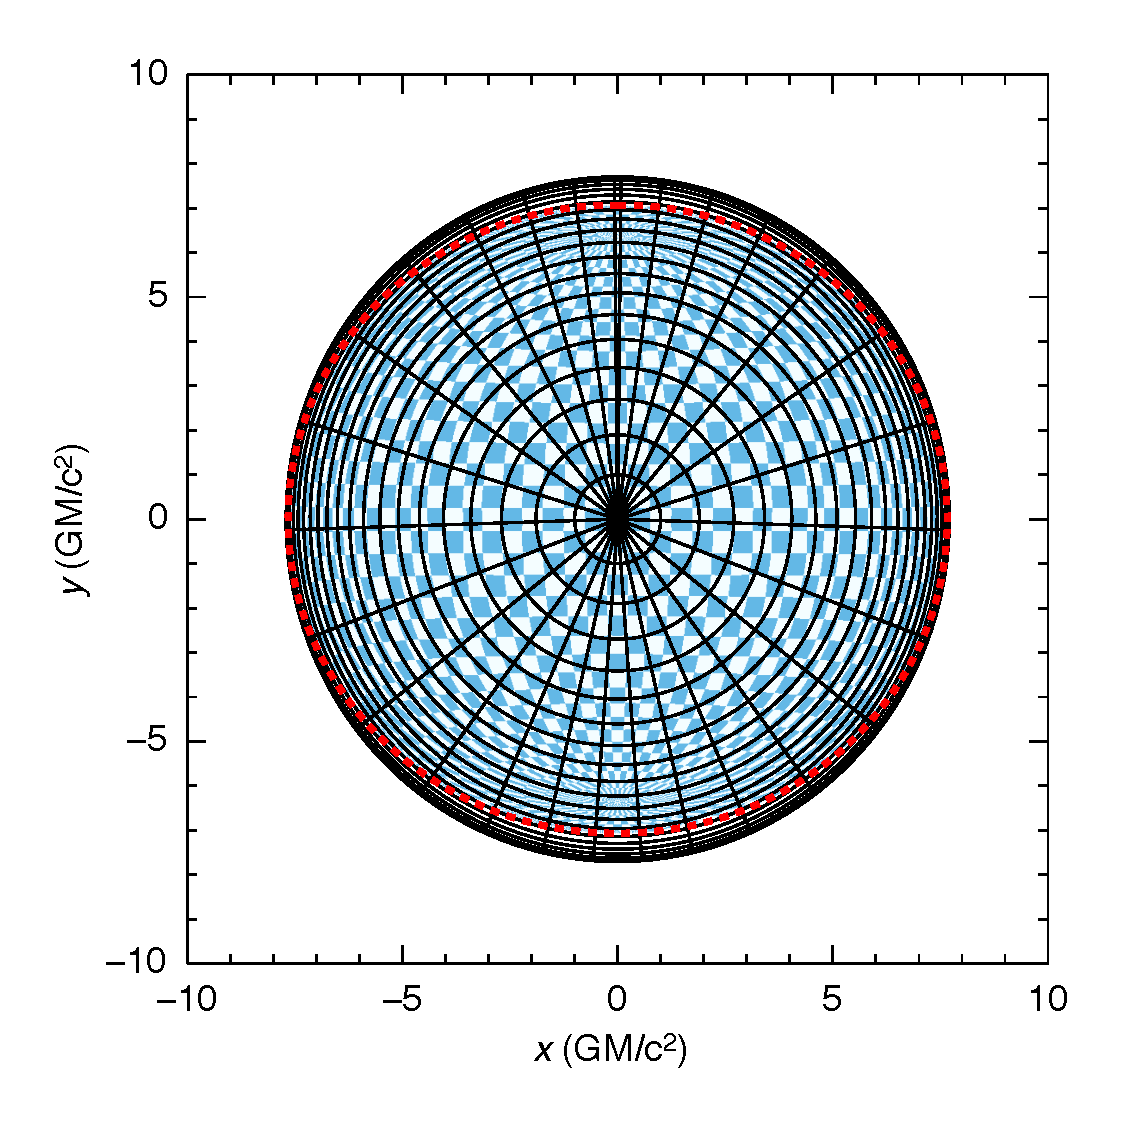
\includegraphics[width=8cm]{figs/fig6a.pdf}
%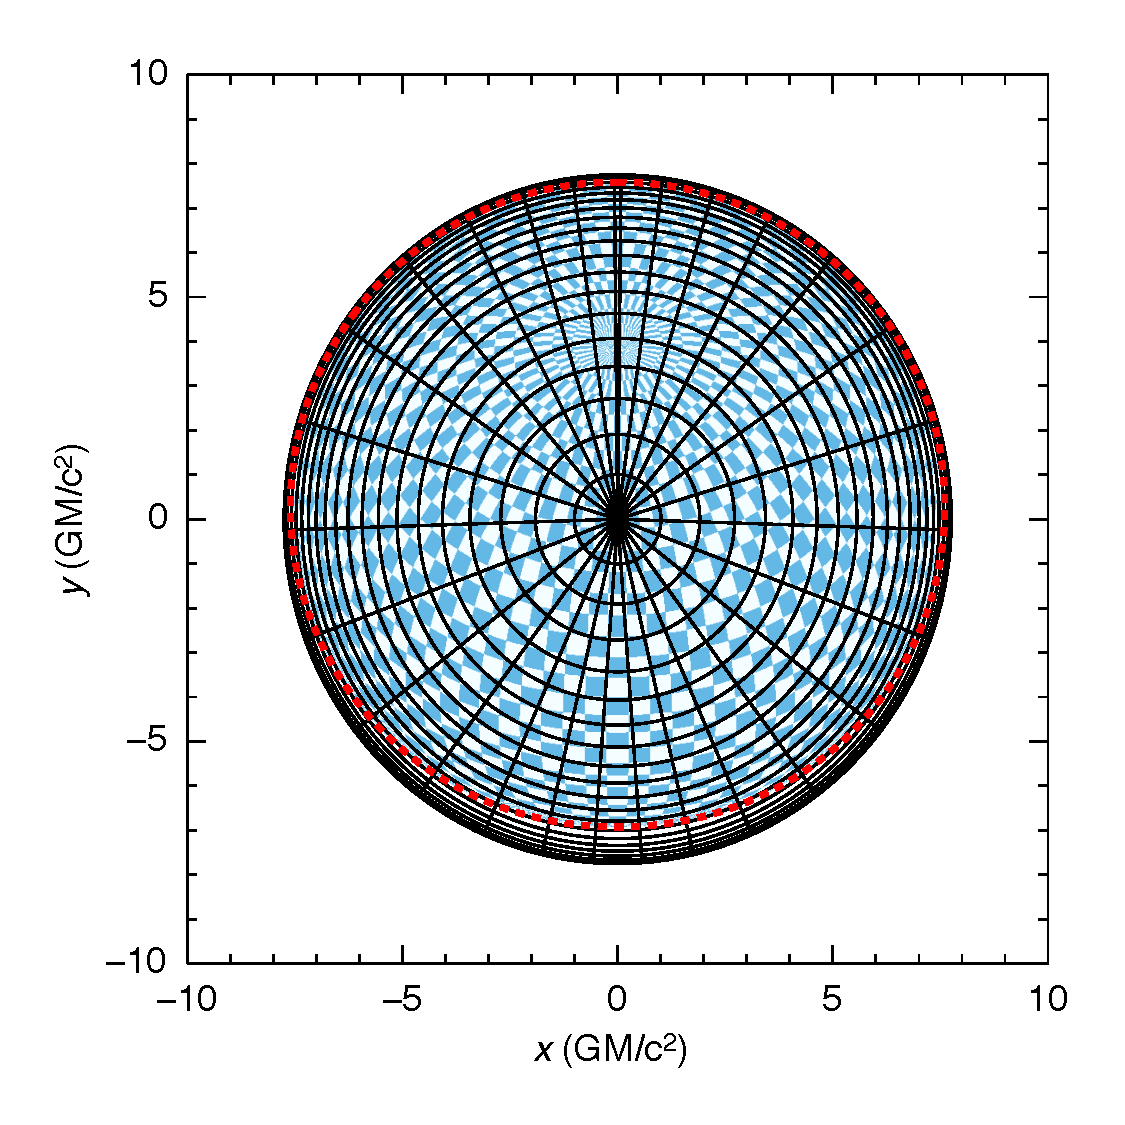
\includegraphics[width=7cm]{figs/fig6b.pdf}
\caption{\label{fig:grid}
Example of a non-equidistant polar grid used in our ray tracing with $N_r = 20$ and $N_{\chi} = 30$ points.
Red dashed line corresponds to the outline of the actual oblate star that is covered with a chess board pattern.
}
\end{figure}


In practice we trace the photons from the image plate at infinity all
the way to the surface of the star by solving the first order
differential equations \eqref{eq:deltatime} - \eqref{eq:deltaphi}
backwards in time.  In addition, we make a change of variable $r
\rightarrow 1/\tilde{x}$ \red{mikä on $\tilde{x}$:n määritelmä?} that will help us by stretching the step when
far from the star and shortening it when coming close to the star
surface.  Here an adaptive stepsize second order Heun's Runge-Kutta
integrator is used with forward Euler's method as
the predictor and trapezoidal method as the corrector.  
All photons that travel
more than $0.95\tilde{x}$ away from the star after a U-turn are
terminated and considered to have missed the star.

Our image plate is defined using a polar coordinate system with a radial
coordinate $b$ (i.e. the impact parameter) and an angular coordinate $\chi$.
We also employ a non-equidistant grid in both coordinates to accommodate
the extra resolution needed around the edges of the star.  Radial
coordinate $b$ is defined using a Gauss-Laguerre abscissae (i.e.
$e^{-b}$-weighted) and the angle coordinate is weighted with a simple
sinusoidal function so that the resolution is increased around the top
and bottom parts where $\chi = 0$ or $\pi$, which is near location of the poles
(see Fig.~\ref{fig:grid}).  By raytracing we then obtain
a mapping between the image plane and the surface of the star, defined
on a grid.
Arbitrary positions in the image plane are 
obtained by a linear interpolation in $(b, \chi)$ space.

For pulse profile calculations where only a small part of the star is
emitting we first search a crude location of the spot on the image plane
and then impose a fine subgrid around it in order to accurately
calculate the flux from this small patch.  The subgrid itself is defined
either in polar grid (by constraining minimum and maximum $\chi$ and
$b$) or in Cartesian image grid (by constraining minimum and maximum
$\hat{x}$ and $\hat{y}$) depenging on the total area covered.  To
calculate the total flux $F(t)$ we then integrate this small subgrid by
using an adaptive multidimensional integration.  The algorithm is based
on a tensor product of nested Clenshaw-Curtis quadrature rules and is
implemented using the \textsc{Cubature} package.



%%%%%%%%%%%%
\section{Comparison \& accuracy}

\subsection{Schwarzschild $+$ Doppler}

To validate the accuracy of the code we did several comparisons with
other methods found in the literature.
The comparison codes propagate photons forward in time, from the surface to the
observer. As such, our code serves a great validation tool for these
codes, since in our code, the photons are propagated backwards in
time.

First, a general comparison
of the ray tracing algorithm with the so-called
Schwarzchild $+$ Doppler approximation \citep[see e.g.][]{PB06} was done.  
For simplicity, we considered only spherical stars was considered here.
Main parameters were: the stellar mass $M = 1.6~\Msun$, the stellar radius $R =
12~\mathrm{km}$, the observer inclination $i = 60^{\circ}$ and the colatitude
of the spot $\theta_{\mathrm{d}} = 50^{\circ}$.  The effective
temperature of the radiation was set to $T_{\mathrm{eff}} =
2~\mathrm{keV}$.  The distance to the source was assumed to be $D =
10~\mathrm{kpc}$.  We defined a circular spot with angular radius $\rho$
either $1$ or $30$ degrees, as measured from the center of the neutron
star.  Here we stress that the spot is defined
using an angle as measured by the co-rotating observer (see eq.
\eqref{eq:rel_cos}).  Hence, the spot is circular in
shape for the co-rotating observer, but not so for the distant static observer.
Angular distribution of radiation either corresponds to Lambert's law,
i.e. isotropic blackbody, with constant intensity or an electron scattering
dominated atmosphere, i.e. Hopf profile.

The light curves are computed in 128 time bins.  Zero time $t = 0$
corresponds to the moment when the spot center crosses the plane
defined by the spin axis and the direction to the observer.  
We computed curves for the five following quantities:
monochromatic photon flux
($\mathrm{ph}\,\mathrm{cm}^{-2}\,\mathrm{s}^{-1}\,\mathrm{keV}^{-1}$) at
the observer energies $E = 2,~6$ and $12~\mathrm{keV}$, bolometric
photon flux ($\mathrm{ph}\,\mathrm{cm}^{-2}\,\mathrm{s}^{-1}$), and the
bolometric energy flux
($\mathrm{erg}\,\mathrm{cm}^{-2}\,\mathrm{s}^{-1}$).


\begin{figure*}
\centering
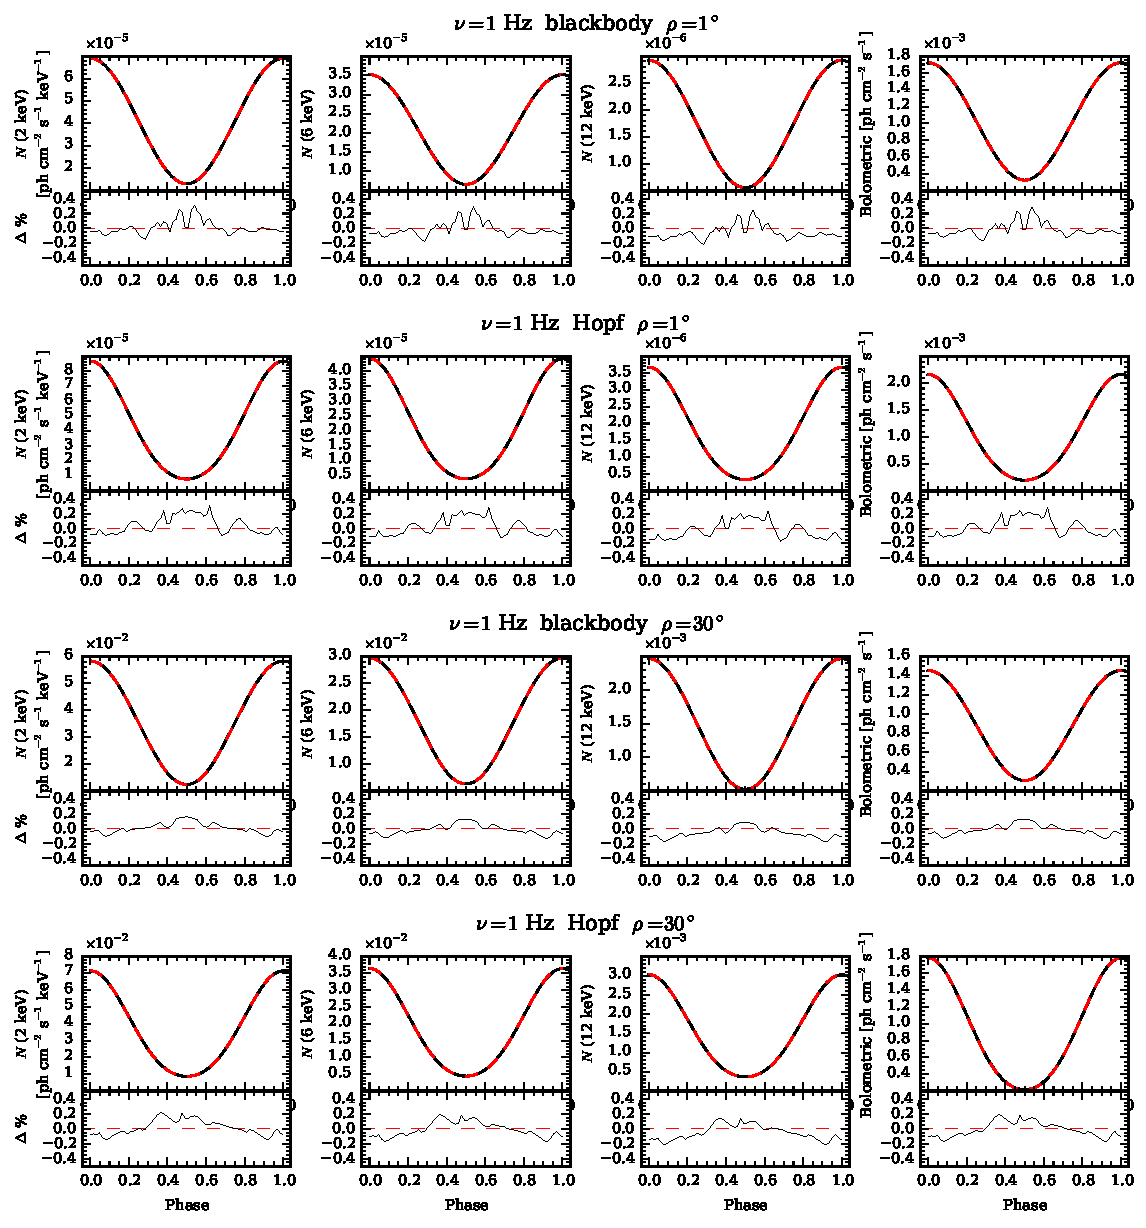
\includegraphics[width=18cm]{figs/fig2a.pdf}
\caption{\label{fig:sch_comp1}
  Light curve comparisons for Schwarzchild spacetime with slowly rotating spherical star ($R = 12~\mathrm{km}$, $M = 1.6~\Msun$, $\nu = 1~\mathrm{Hz}$, $i = 60^{\circ}$, $\theta_s = 50^{\circ}$, $\rho = 1^{\circ}$, and $T_{\mathrm{eff}} = 2~\mathrm{keV}$) emitting according to Lambert law or Hopf profile with spot size either $1$ or $30$ degrees.
  Black solid line shows the pulse profiles computed using the forward-in-time code by J. Poutanen and red dashed line is a profile computed with the code presented here.
  The lower panel shows the residuals as $\Delta = (\mathrm{model_{JP}}/\mathrm{model} -1) \times 100\%$.
}
\end{figure*}

\begin{figure*}
\centering
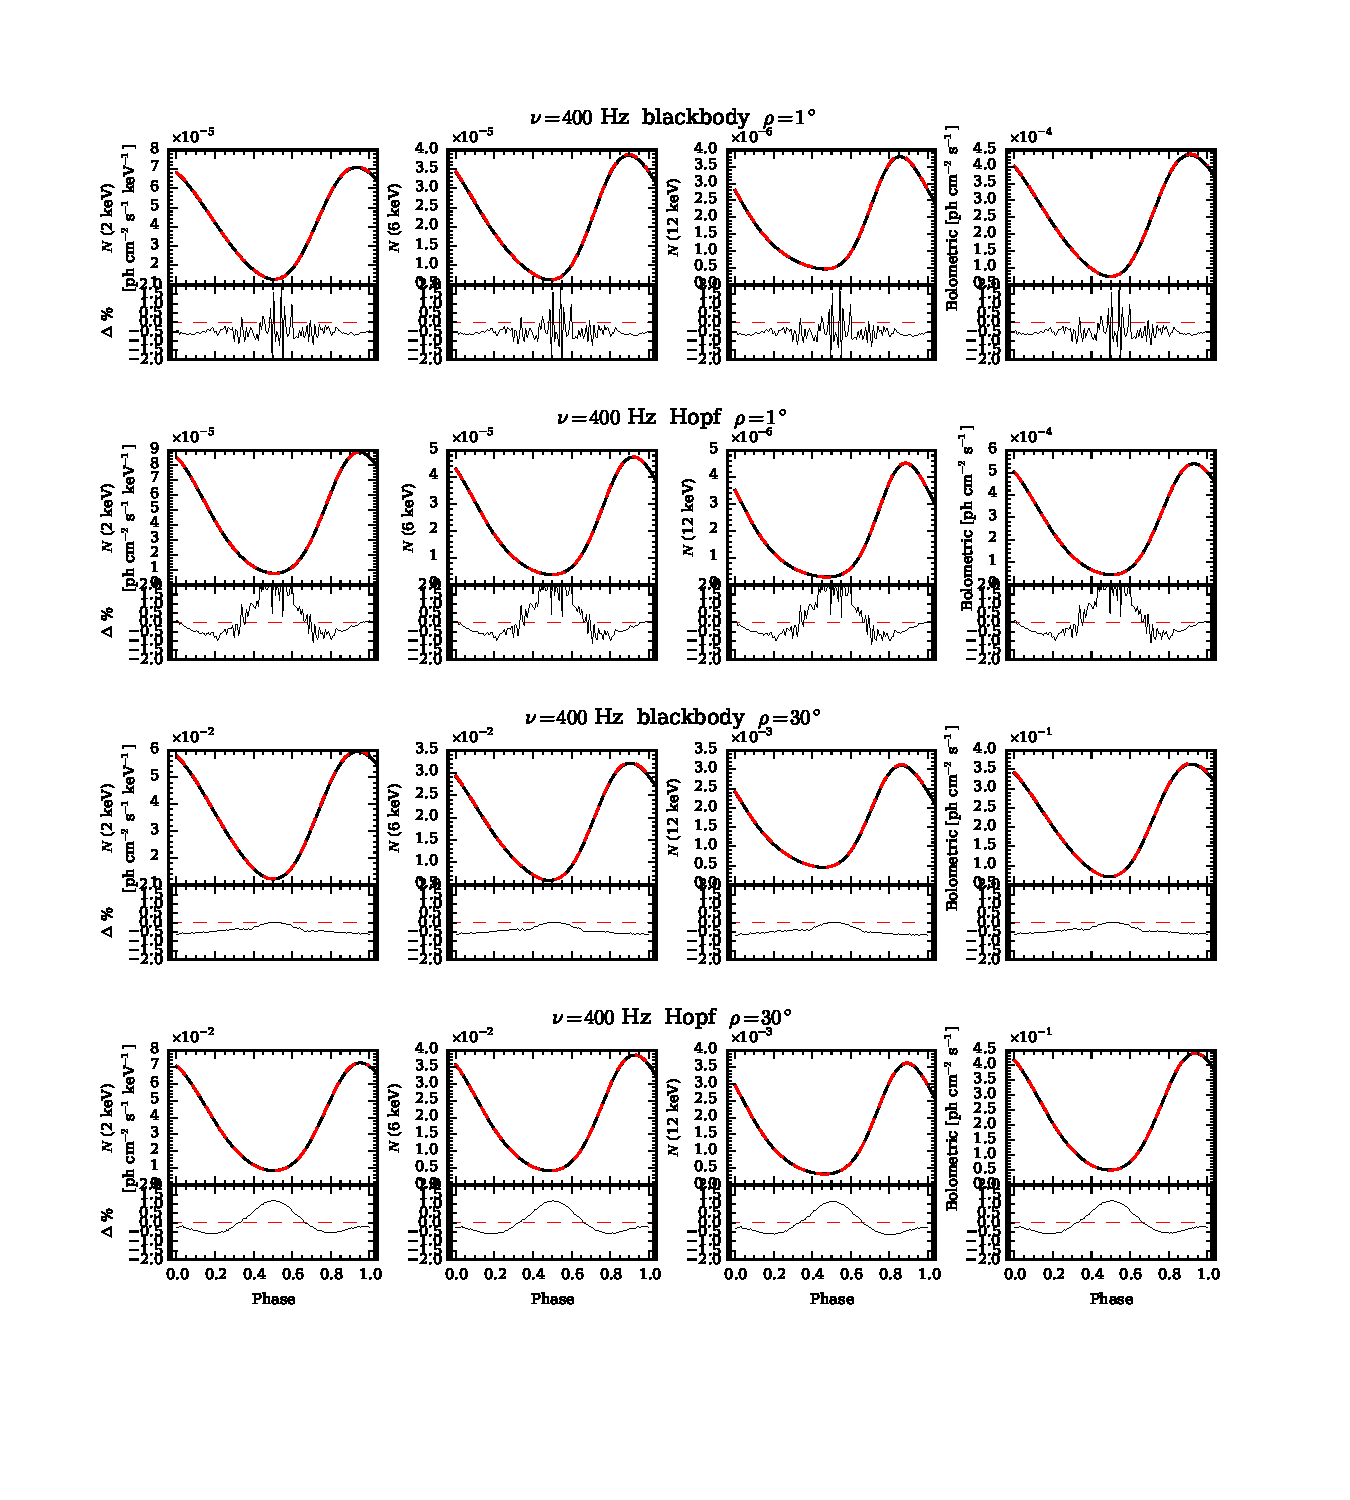
\includegraphics[width=18cm]{figs/fig2b.pdf}
\caption{\label{fig:sch_comp400}
  Light curve comparisons for Schwarzchild spacetime with rapidly rotating spherical star ($\nu = 400~\mathrm{Hz}$).
  Otherwise the parameters and symbols are the same is in Fig.~\ref{fig:sch_comp1}.
}
\end{figure*}


Comparison of these lightcurves are shown in Fig.~\ref{fig:sch_comp1} for slowly rotating star ($1$ Hz) and in Fig.~\ref{fig:sch_comp400} for fast rotation ($400$ Hz).
In practice, comparing the profiles for slow rotation only tests our ray tracing routines because special relativistic effects (Doppler boosting, angle aberration and so on) are negliglible.
Overall agreement of the two different methods is excellent and from here a baseline accuracy of about $<0.2\%$ relative error is constrained for the mapping of quantities between image plane and star's surface.
Similarly, when rotation is increased and special relativistic effects start to play a role we are able to reproduce the pulse profiles usually down to $<0.3\%$ relative error.
No large deviation between isotropic and Hopf profile is detected either, indicating that the emission angle is also computed correctly.

\subsection{Oblate Schwarzchild $+$ Doppler}

Next we compare emission from oblate surfaces.
The surface here is defined using the radius function \eqref{eq:radf} but the star is still embbed in a symmetric \sch spacetime.
The parameters used are equatorial radius $R_{\mathrm{eq}} = 12~\mathrm{km}$ (in the usual \sch metric), star mass of $M = 1.4~\Msun$, extreme rotational frequency $\nu = 700~\mathrm{Hz}$, observer inclination $i=45^{\circ}$, and spot angular size of $\rho = 10^{\circ}$
Effective temperature of the radiation is again taken to be $T_{\mathrm{eff}} = 2~\mathrm{keV}$ and the distance $D = 10~\mathrm{kpc}$.
Here the spot size is again defined in the co-rotating \textit{spherical} coordinate system on top of a unit sphere and is then projected to the oblate inclined surface.
To trace the effects of the changing surface we consider the spot in three different locations at colatitudes of $\theta_{\mathrm{S}} = 18^{\circ}$, $45^{\circ}$, and $90^{\circ}$.
Additionally for $\theta_{\mathrm{S}} = 90^{\circ}$ when the spot is on the equator we observer a full eclipse in the light curve.
This imposes a serious test for both of the codes as the gradually more and more blocked spot is also seen from a very shallow angle before disappearing and appearing again.
We note that when integrating flux from the spot in the image plane, a polar subgrid is extremely useful just before the eclipse as the impact parameter can vary only by a $\sim1\%$ before the spot is hidden behind the star.
Attaining a similar resolution in a Cartesian subgrid would then need far more integrand evaluations as the spot is seen from a very shallow angle.

%\begin{figure*}
%\centering
%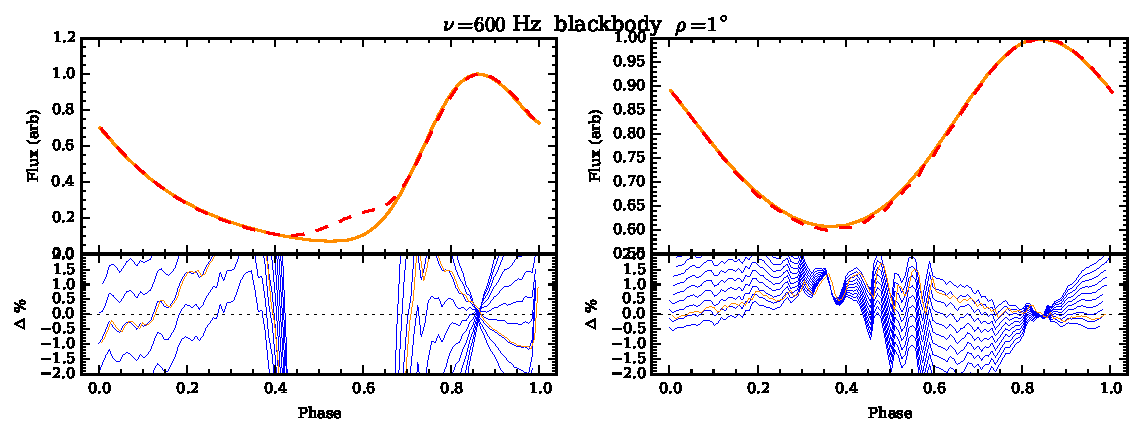
\includegraphics[width=16cm]{figs/fig3.pdf}
%\caption{\label{fig:sch_obl}
%  Bolometric energy flux comparisons for oblate Schwarzchild approximation with rapidly rotating star ($R_{\mathrm{eq}} = 16.4~\mathrm{km}$, $M = 1.4~\Msun$, $\nu = 600~\mathrm{Hz}$, and $\rho = 1^{\circ}$).
%  Left panel shows a pulse profile as compared to fig. 3 in \cite{MLCB07} with $i = 70^{\circ}$ and $\theta_s = 49^{\circ}$.
%  The spherical star is taken to have $R(49^{\circ}) = 15.1~\mathrm{km}$.
%  Right panel can be compared against fig. 4 in \cite{MLCB07} with $i = 20^{\circ}$ and $\theta_s = 41^{\circ}$
%  In this case, the spherical star has $R(41^{\circ}) = 14.8~\mathrm{km}$.
%}
%\end{figure*}


\begin{figure*}
\centering
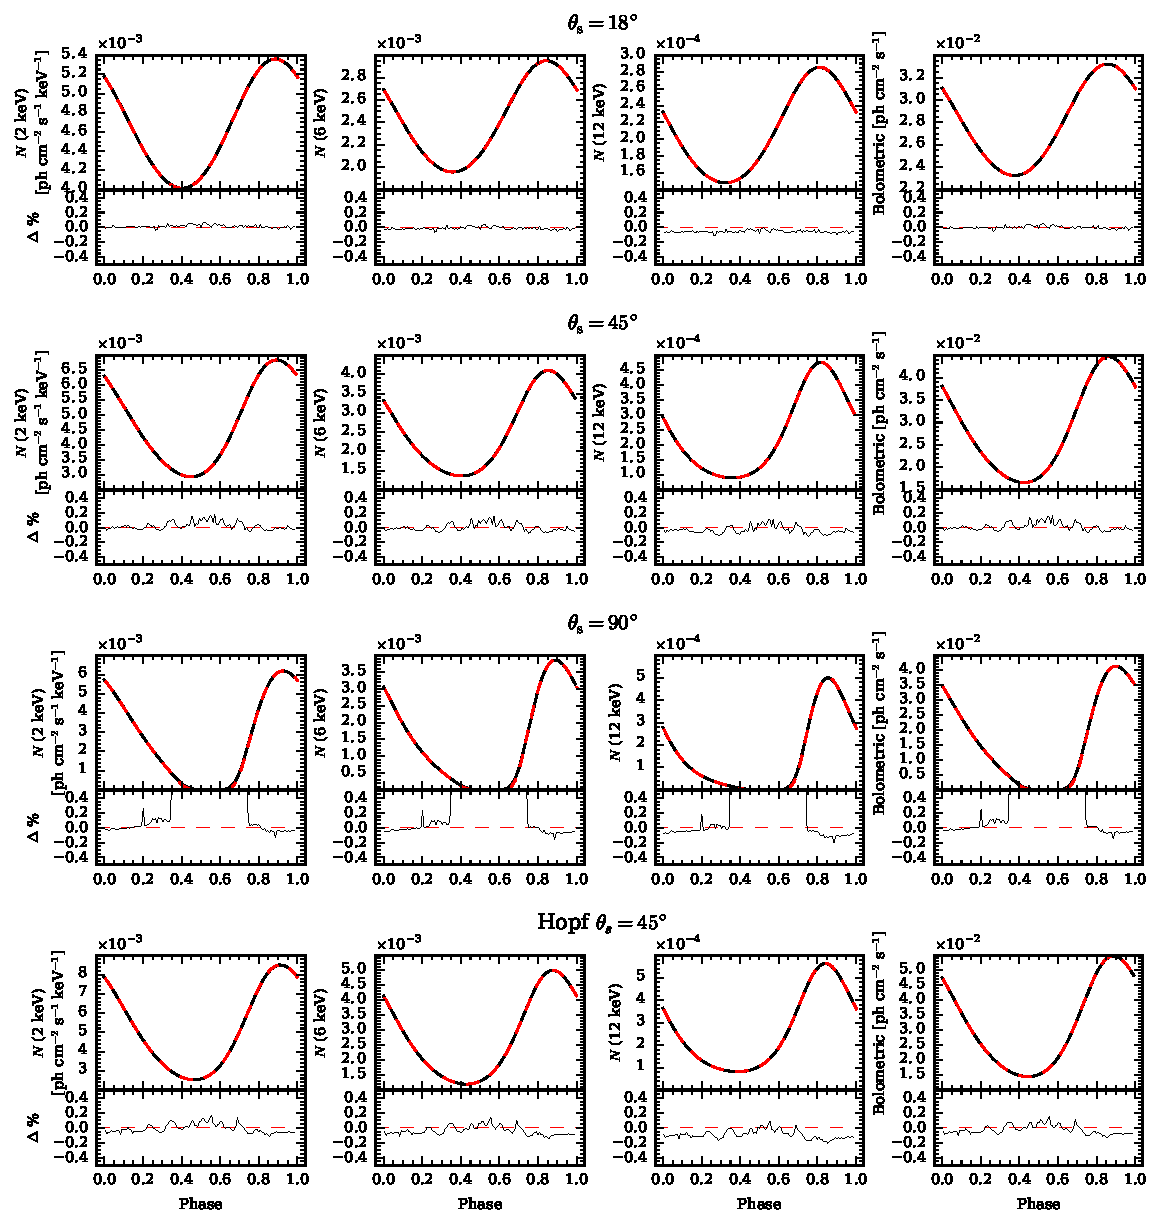
\includegraphics[width=18cm]{figs/fig4.pdf}
\caption{\label{fig:osch_comp700}
  Light curve comparisons for oblate Schwarzchild spacetimes with three different spot colatitudes: $\theta_{\mathrm{c}} = 18^{\circ}$, $45^{\circ}$ and $90^{\circ}$.
  Parameters of the star, spot and observer are: $R_{\mathrm{eq}} = 12.0~\mathrm{km}$, $M = 1.4~\Msun$, $\nu = 700~\mathrm{Hz}$, $i = 45^{\circ}$ and $\rho = 10^{\circ}$.
  Otherwise the parameters and symbols are the same is in Fig.~\ref{fig:sch_comp1}.
  }
\end{figure*}

Comparison of the oblate lightcurves are shown in Fig.~\ref{fig:osch_comp700}.






\subsection{Hartle-Thorne -like spacetimes}

%\begin{figure*}
%\centering
%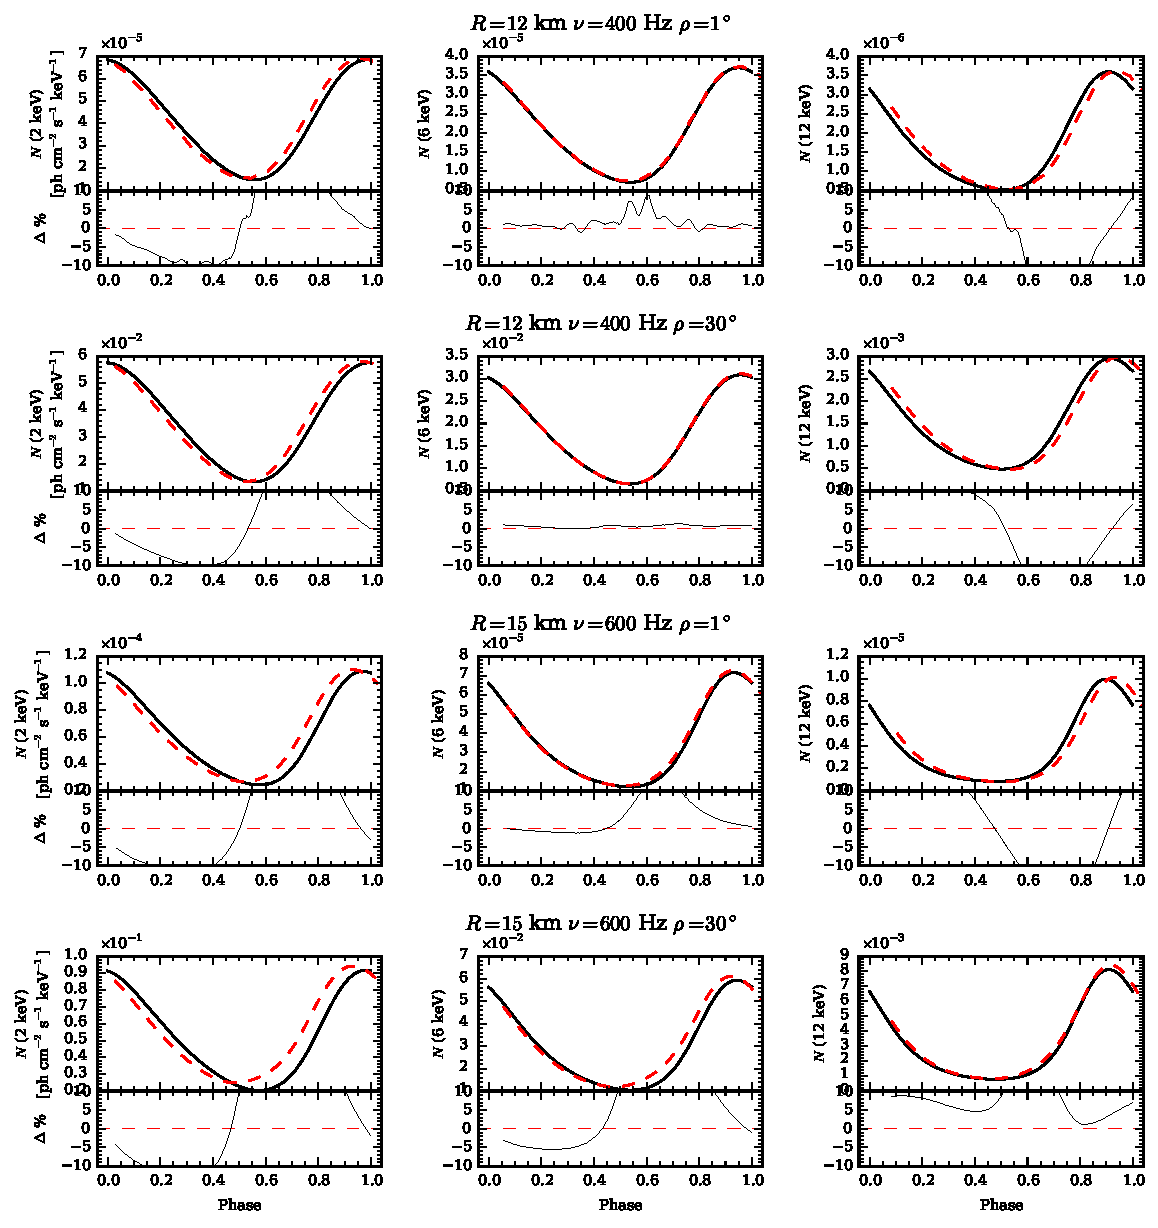
\includegraphics[width=18cm]{figs/fig5.pdf}
%\caption{\label{fig:sch_comp400}
%  Light curve comparisons for Hartle-Thorne spacetime with rapidly rotating oblate stars.
%}
%\end{figure*}



\subsection{Carter's constant splitting}

\begin{figure*}
\centering
\includegraphics[width=18cm]{figs/popiha/casual_400pts_16m_12km_400hz_15inc.pdf}
\includegraphics[width=18cm]{figs/popiha/casual_400pts_16m_12km_400hz_45inc.pdf}
\includegraphics[width=18cm]{figs/popiha/casual_400pts_16m_12km_400hz_75inc.pdf}
\includegraphics[width=18cm]{figs/popiha/extreme_400pts_14m_15km_600hz_15inc.pdf}
\includegraphics[width=18cm]{figs/popiha/extreme_400pts_14m_15km_600hz_45inc.pdf}
\includegraphics[width=18cm]{figs/popiha/extreme_400pts_14m_15km_600hz_75inc.pdf}
\caption{\label{fig:H_C1_C2}
  Error in ray tracing.
  }
\end{figure*}







%\section{Conclusions}
\section*{Acknowledgments}

\bibliographystyle{apj}
\bibliography{allbib}

%\begin{thebibliography}
%\end{thebibliography}


\clearpage
\appendix

\section{Additional stuff about elliptic integrals and so on}

After separating the equation \eqref{eq:hamjac} with the help of the
Carter's constant $\Ca$, we get the remaining four-momentum components
\be\label{eq:pr}
p_r = \pd_r S = e^{-2\nub} \left( (E-L_z \omega)^2 - \frac{\mathcal{C}}{e^{-2\nub} r^2} \right)^{1/2} = \mathcal{R}(r)
\ee
and
\be\label{eq:ptheta}
p_{\theta} = \pd_{\theta} S = e^{\mu} \left( \mathcal{C} - \frac{L_z^2}{\sin^2 \theta} \right)^{1/2} = \Theta(\theta).
\ee
Now, in addition to our pre-defined constants $E$ and $L_z$, we have a
new constant of motion $\Ca$, for which
\be
\frac{\pd S}{\pd \mathcal{C}} = \frac{1}{2} \int^r \frac{1}{\sqrt{\mathcal{R}}} \frac{\pd \mathcal{R}}{\pd \mathcal{C}} dr + \frac{1}{2} \int^{\theta} \frac{1}{\sqrt{\Theta}} \frac{\pd \Theta}{\pd \mathcal{C}} d\theta = 0.
\ee 
After substitution and cancellation of terms the relation leads to elliptic integrals of the form
\begin{align}\begin{split}\label{eq:Lz_C_rel}
 \int^r dr e^{\nub} & r^{-2} \left( (E-L_z\omega)^2 - \frac{\mathcal{C}}{e^{-2\nub} r^2} \right)^{-3/4}  = \\
& \int^{\theta} d\theta e^{\mu/2} \left(\mathcal{C} - \frac{L_z^2}{\sin^2 \theta} \right)^{-3/4}
\end{split}\end{align}
connecting our three constants of motion.
This can be refined further
when we remember that $e^{\mu} \approx 1$, i.e. constant without any $\theta$ dependency. 
With this in mind, we can write
\be
\int^{\theta} d\theta e^{\mu/2} \left(\mathcal{C} - \frac{L_z^2}{\sin^2
\theta} \right)^{-3/4} = -\frac{e^{\mu/2} L_z}{\mathcal{C} (\mathcal{C}-L_z^2)^{1/4}} [ \Pi(n; \alpha, -1)+\Pi(-n;\alpha, -1)],
\ee
where $\Pi$ is the incomplete elliptic integral of the third kind with
parameters $n = \sqrt{1-L_z^2/\mathcal{C}}$ as the elliptic
charasteristic and the angle $\alpha$ defined as $\sin^4 \alpha =
(\mathcal{C}-L_z^2 \csc^2 \theta)/(\mathcal{C}-L_z^2))$ with elliptic
modulus of $-1$.


\section{Special case: equatorial rays}
If we limit ourselves to the equatorial plane ($\theta=\pi/2$ reflection symmetry) the bending equations are simplified tremendously due to the loss of four-momentum component along the $\hat{\theta}$ direction.
The general coordinates of a photon are defined as $x^{\alpha} = (x^{t}, x^{r}, x^{\theta}, x^{\phi})$ and the four-velocity is obtained from $dx^{\alpha}/d\lambda$ through affine parameter $\lambda$.
Again, due to the two Killing vectors $k^{\alpha}$ and $m^{\alpha}$ we now set our constants directly to $u_{t} = 1$ and $u_{\phi} = b$, where $b$ is an impact parameter defined more thoroughly later on.
In the equatorial plane a dual of the four-velocity is then $u_{\alpha} = (1, u_{r}, 0, b)$.
Finally, from $x^{\alpha}x_{\alpha} = 0$ we can solve the $u_{r}$ component to be
\be
u_{r} = e^{-2\nub}\sqrt{(1-b\omega)^2 - e^{2\nub}\frac{b^2}{r^2}} 
\ee

The emission angle $\alpha$ is easily obtained by using the vector notation
\be
\tan \alpha = \frac{(u^{\phi}u_{\phi})^{1/2}}{(u^ru_r)^{1/2}}
\ee
yielding
\begin{align}\begin{split}
\cos \alpha = & 1 + (e^{-2\nub}r^2\omega^2 -1) \times \\
            & \left( 1+b\omega - \sqrt{(1+b\omega)^2 - \left(\frac{b}{e^{-\nub}r}\right)^2} \right),
\end{split}\end{align}
which reduces to
\be
\cos \alpha = \sqrt{1-\left( \frac{b}{e^{-\nub_0}r} \right)^2},
\ee
in the limit of no rotation $\omega \rightarrow 0$. This corresponds to
the solution in a \sch space-time when we remember that $e^{\nub_0} = (1-\rg/R)$.



\end{document}
